\chapter{Appendix}

\begin{figure}
    \centering
    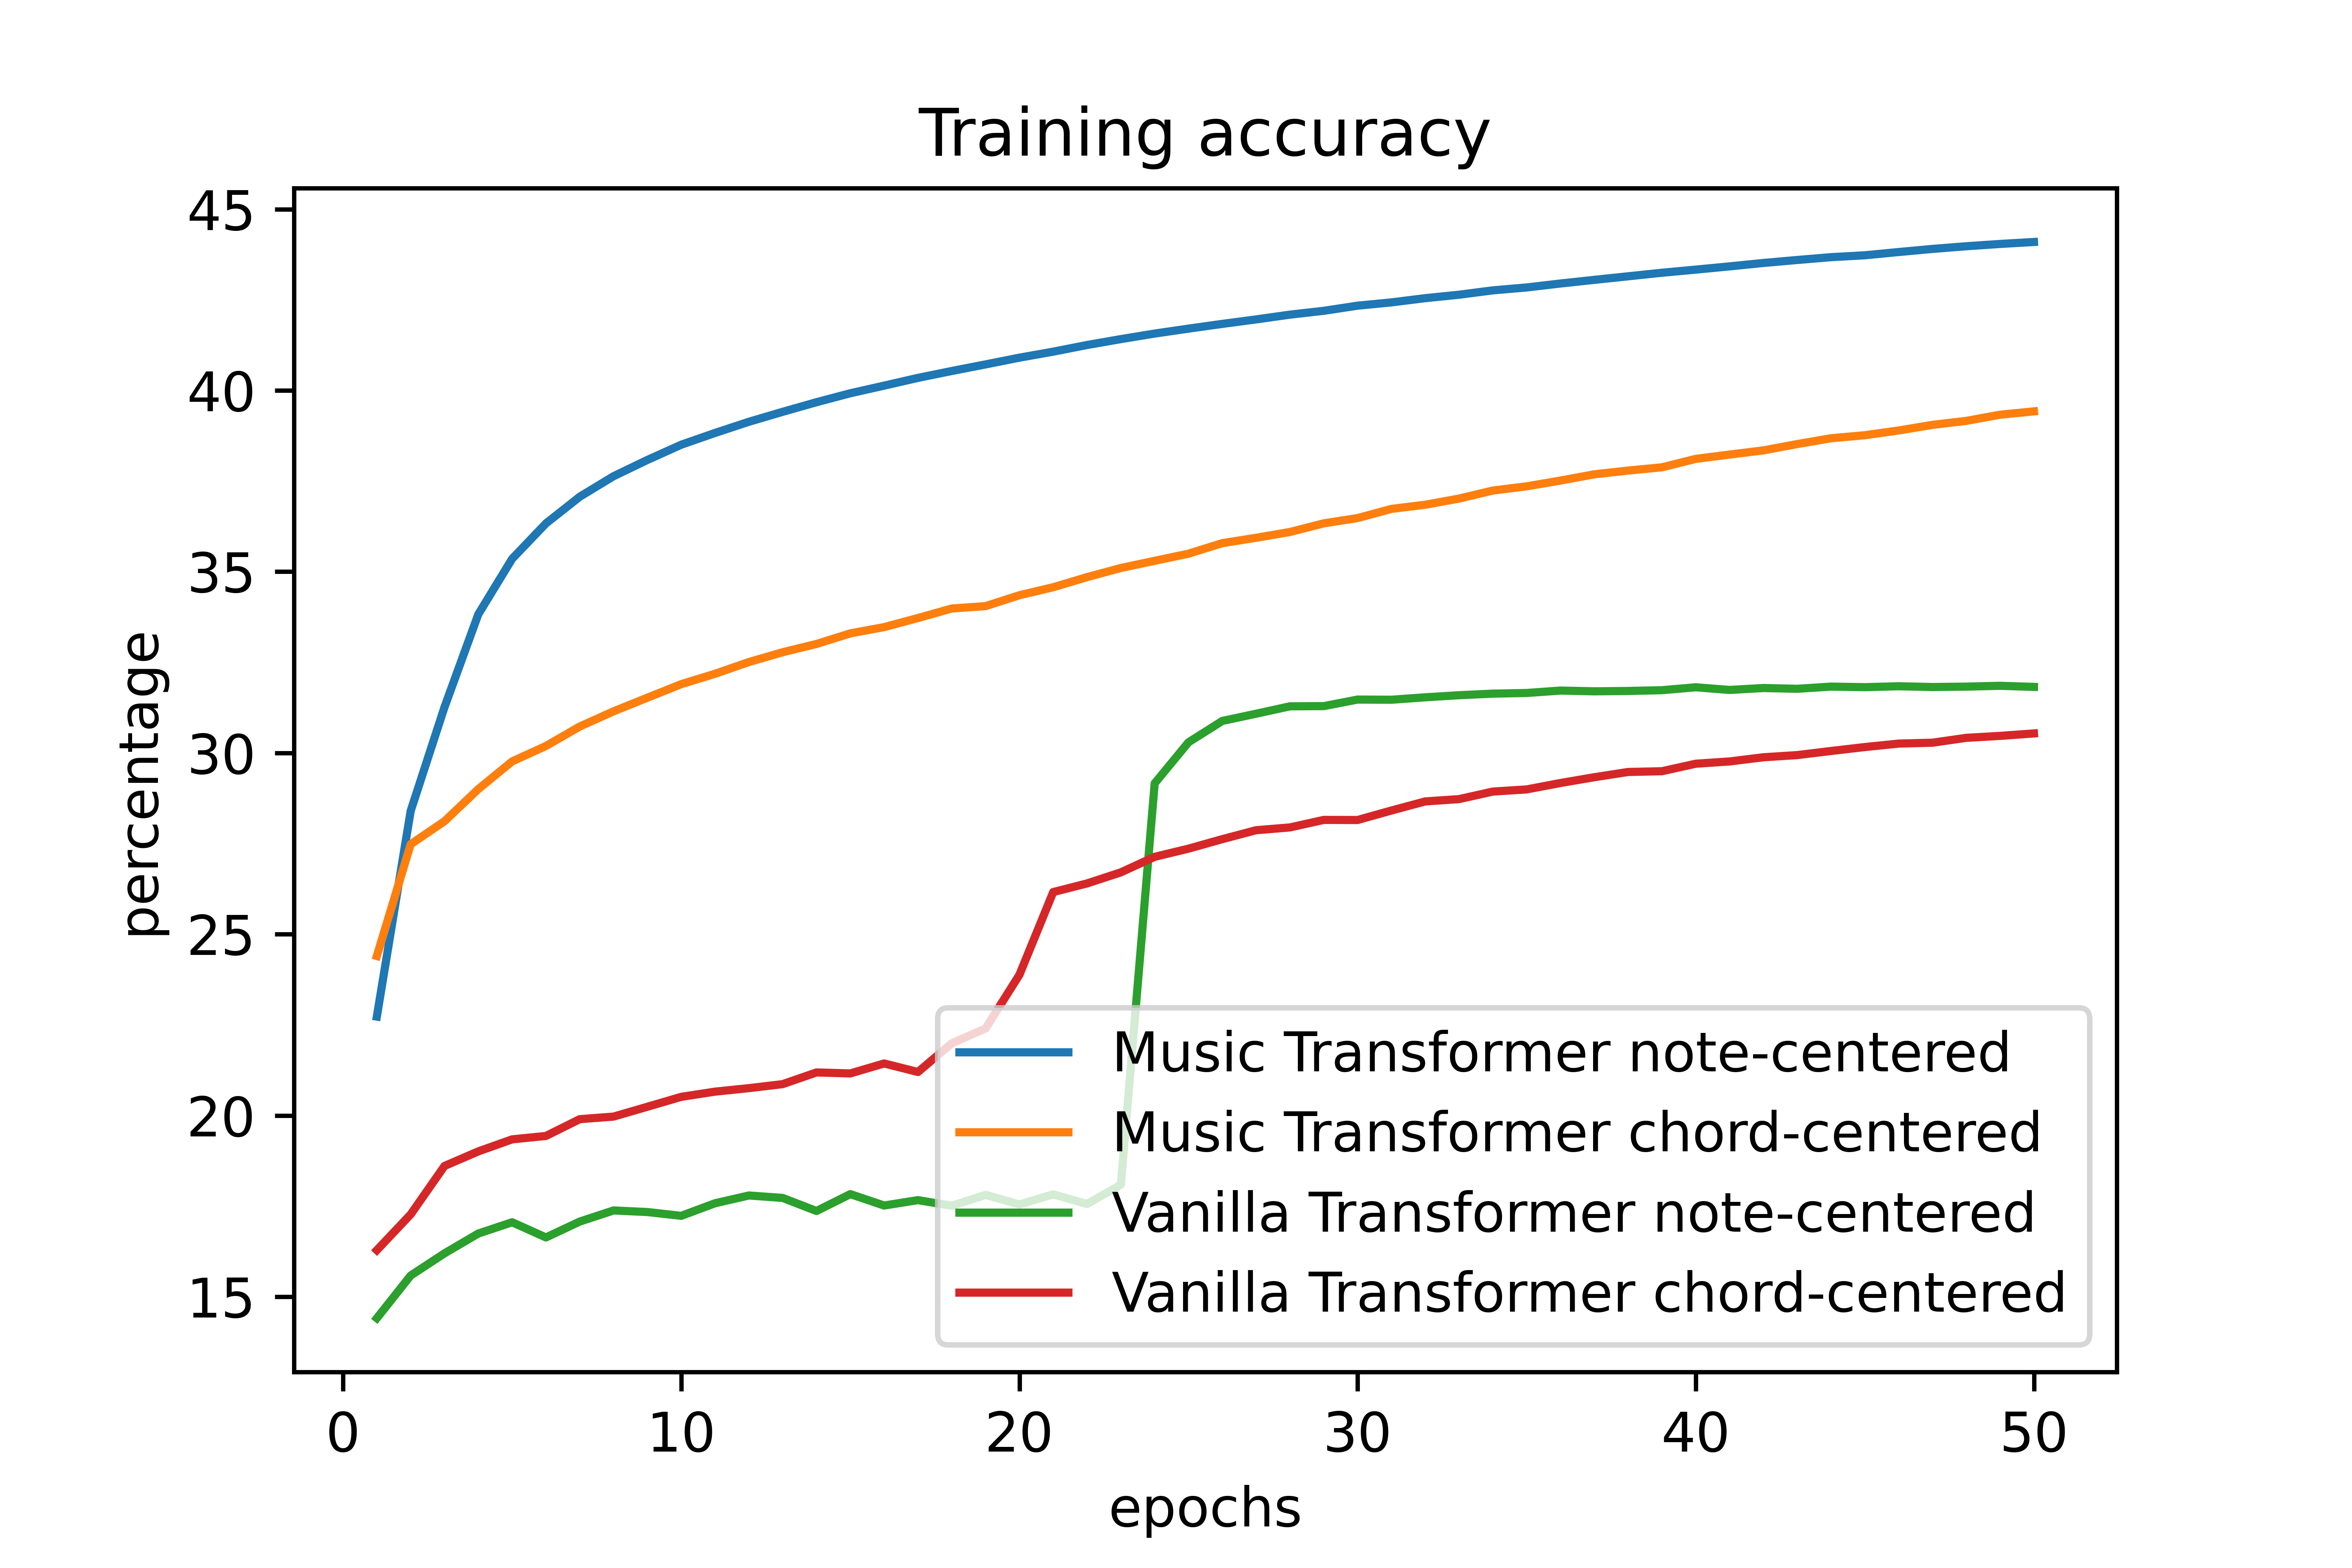
\includegraphics[width=0.8\textwidth]{assets/training-accuracy}
    \caption{~Accuracy of models on training set}\label{fig:appendix-training-accuracy}
\end{figure}
\begin{figure}
    \centering
    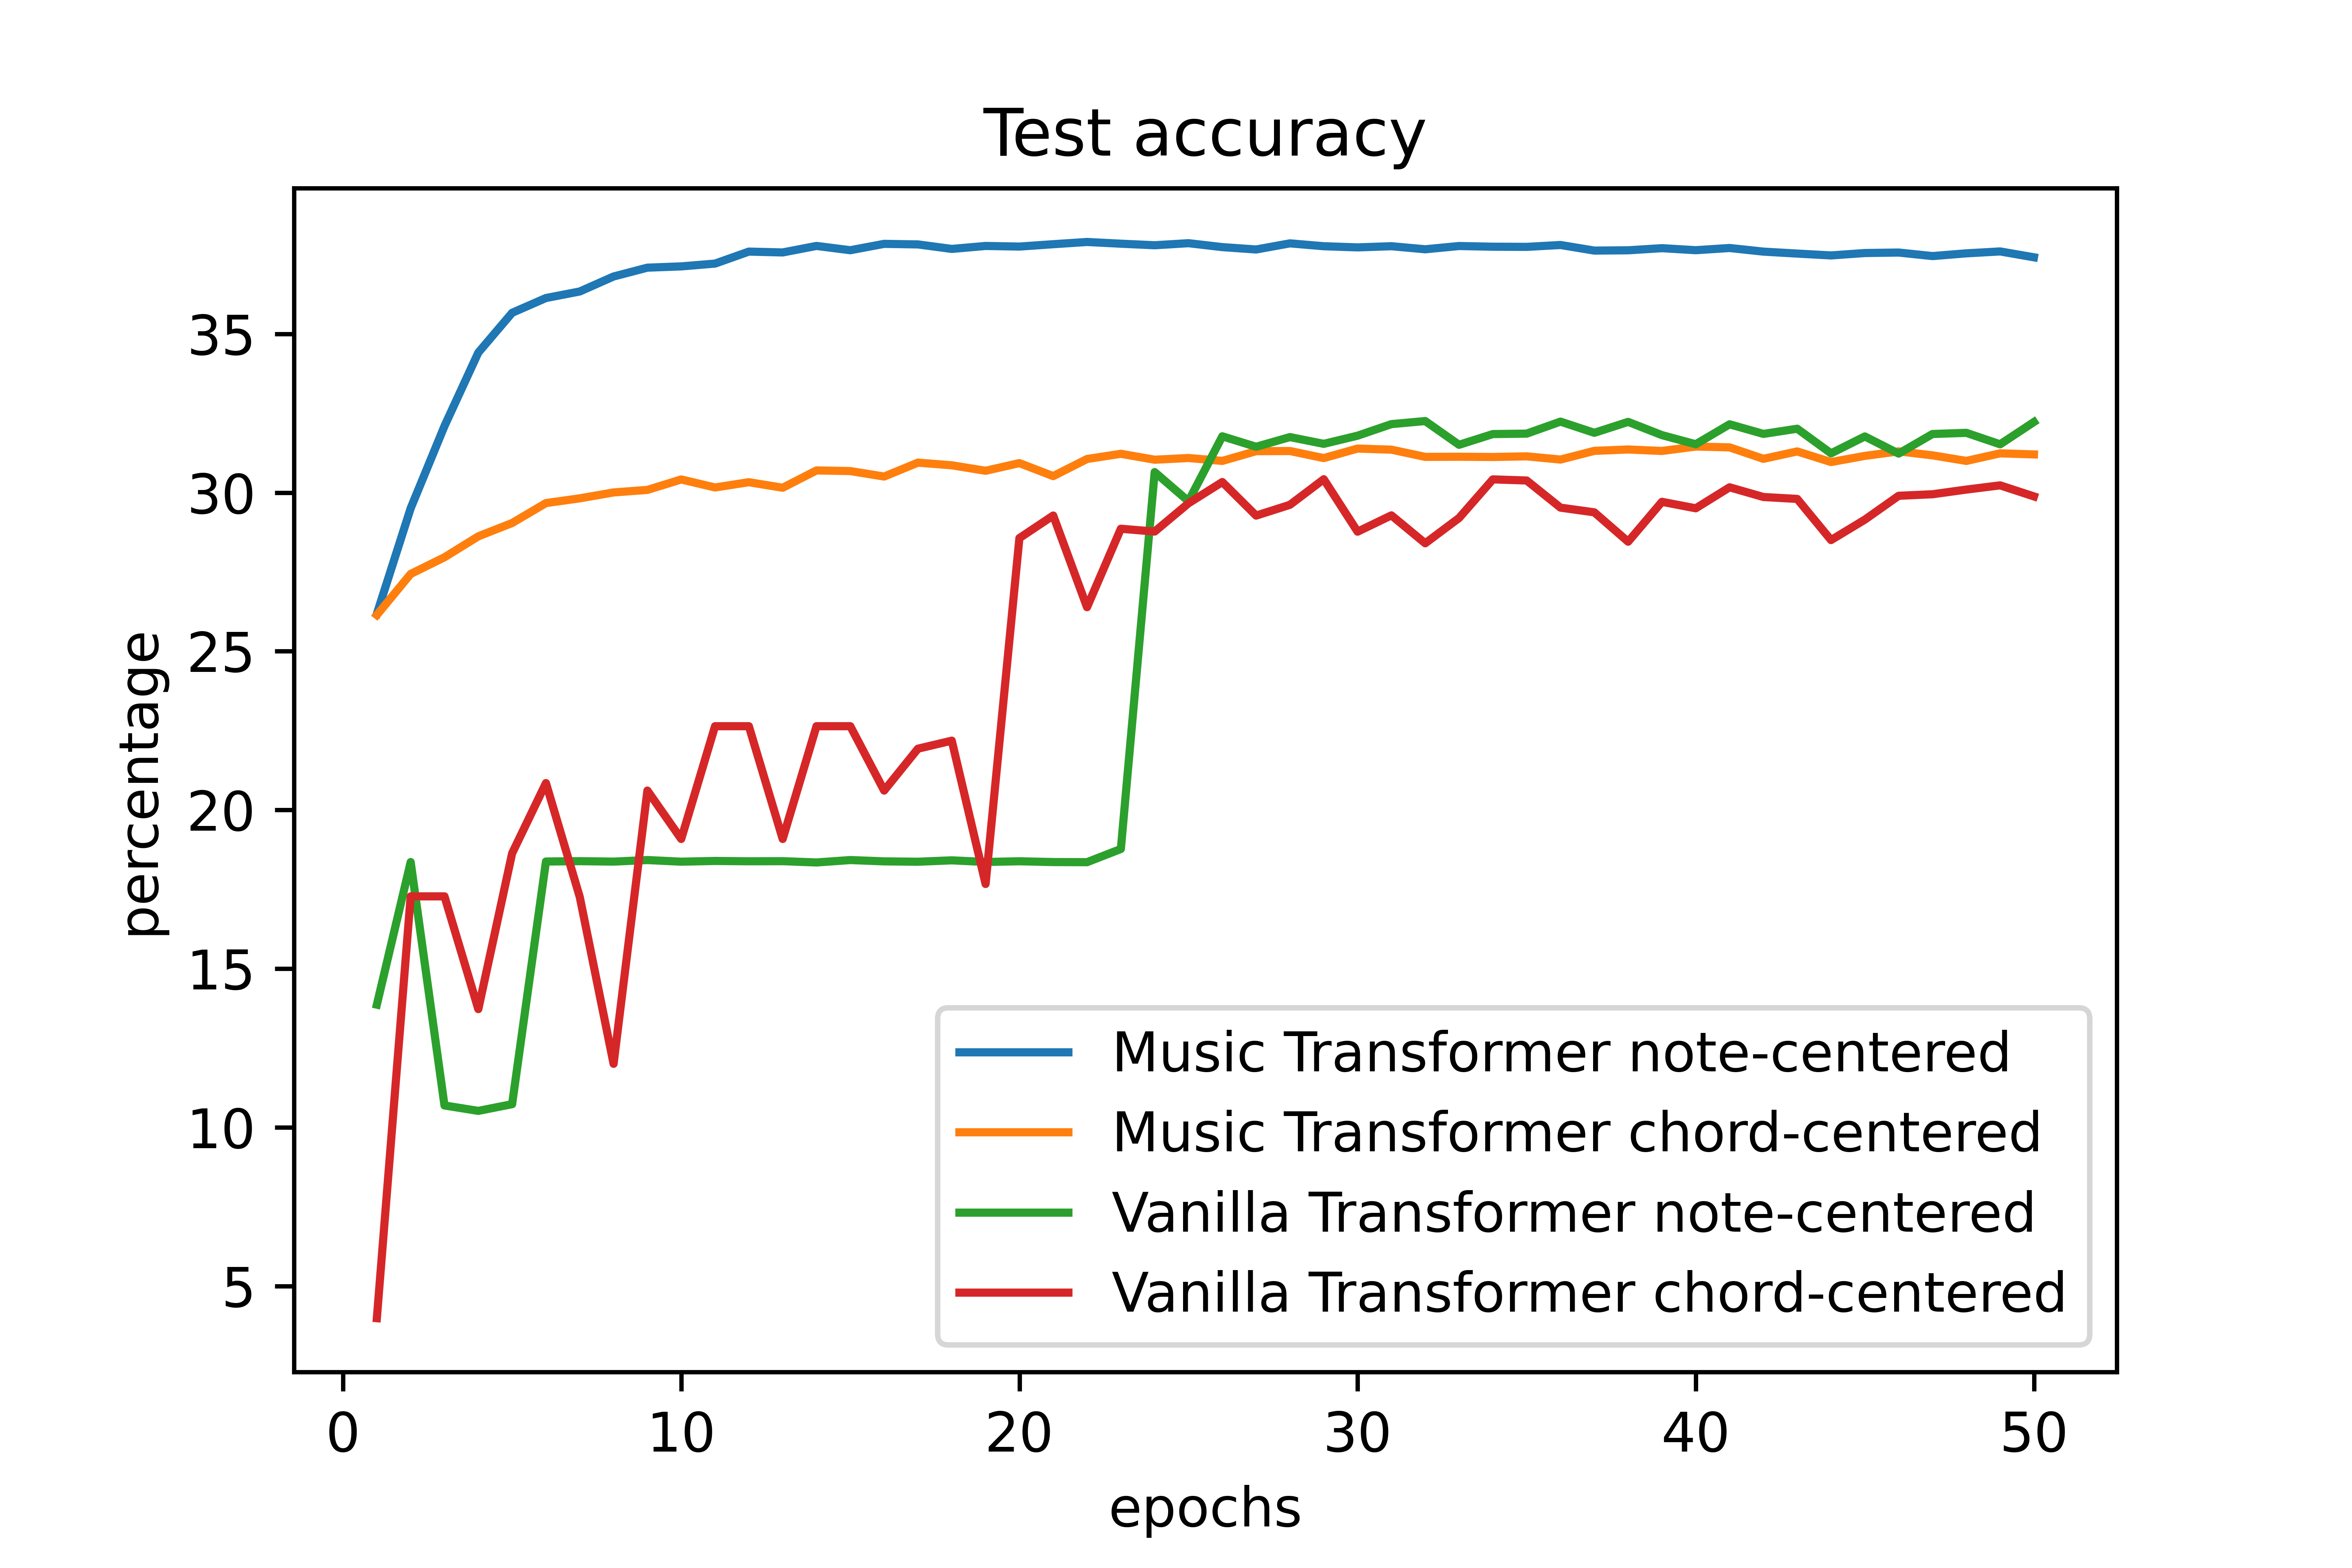
\includegraphics[width=0.8\textwidth]{assets/test-accuracy}
    \caption{~Accuracy of models on test set}\label{fig:appendix-test-accuracy}
\end{figure}

\begin{figure}
    \centering
    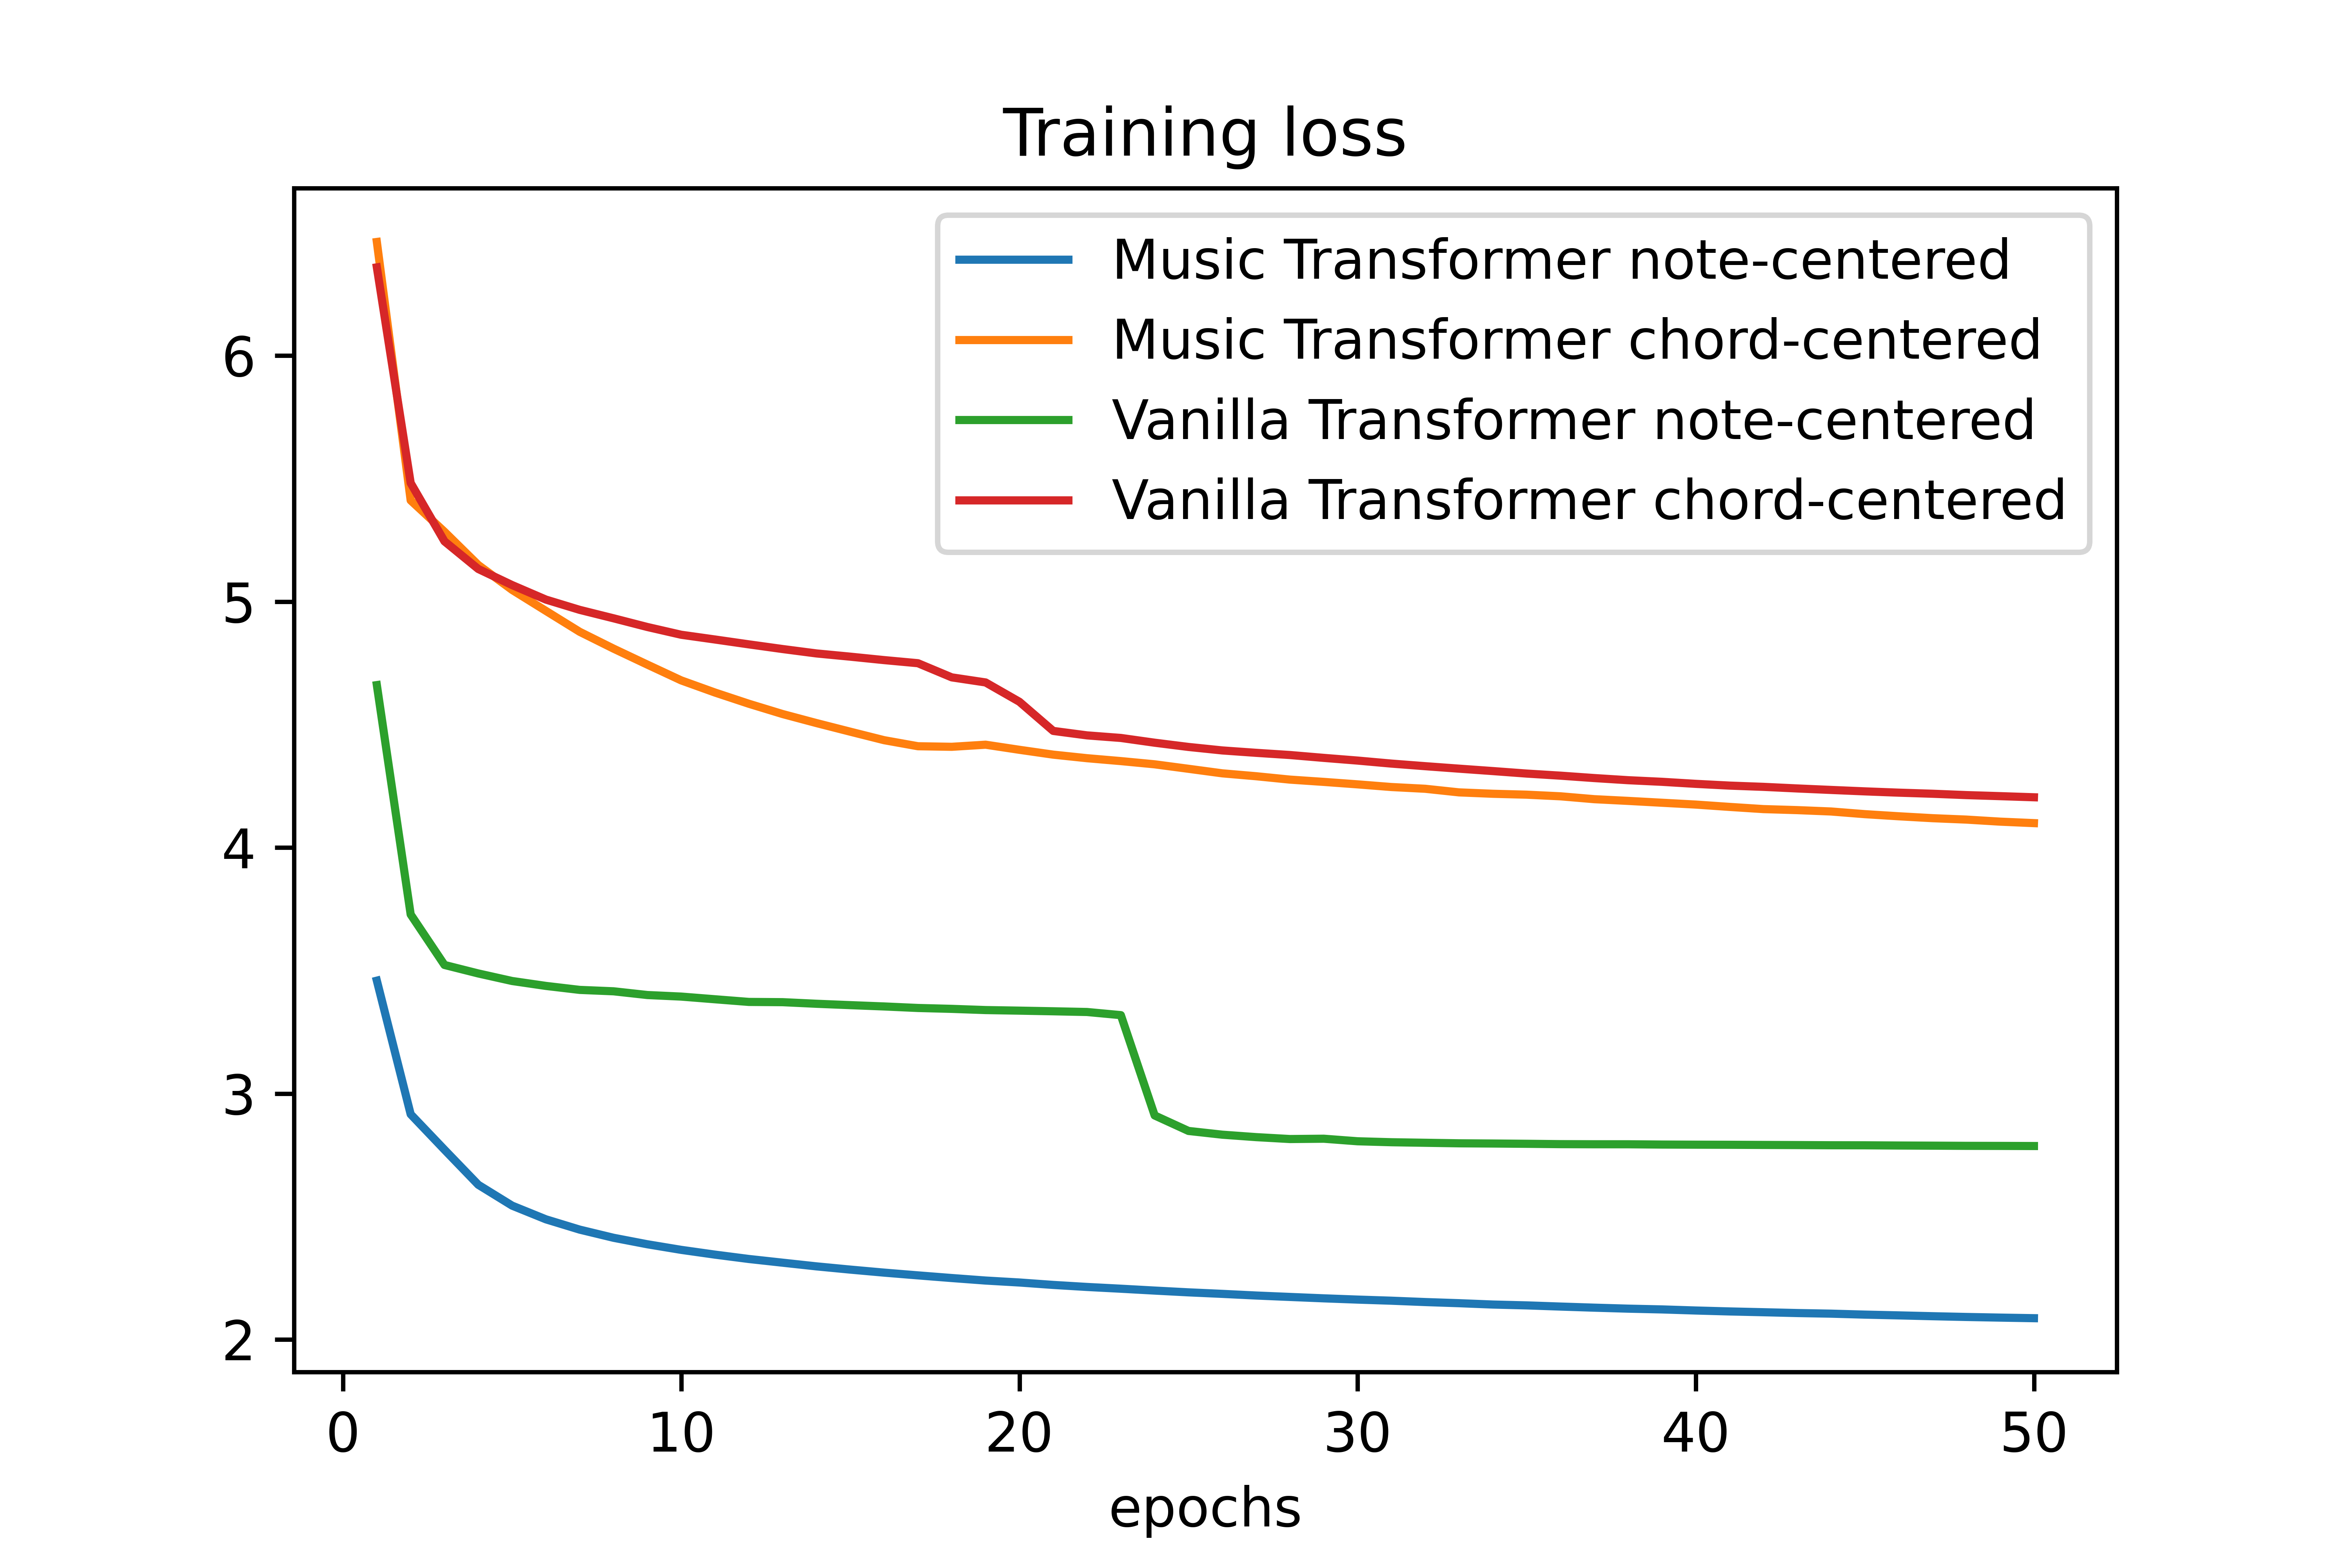
\includegraphics[width=0.8\textwidth]{assets/training-loss}
    \caption{~Loss of models on training set}\label{fig:appendix-training-loss}
\end{figure}
\begin{figure}
    \centering
    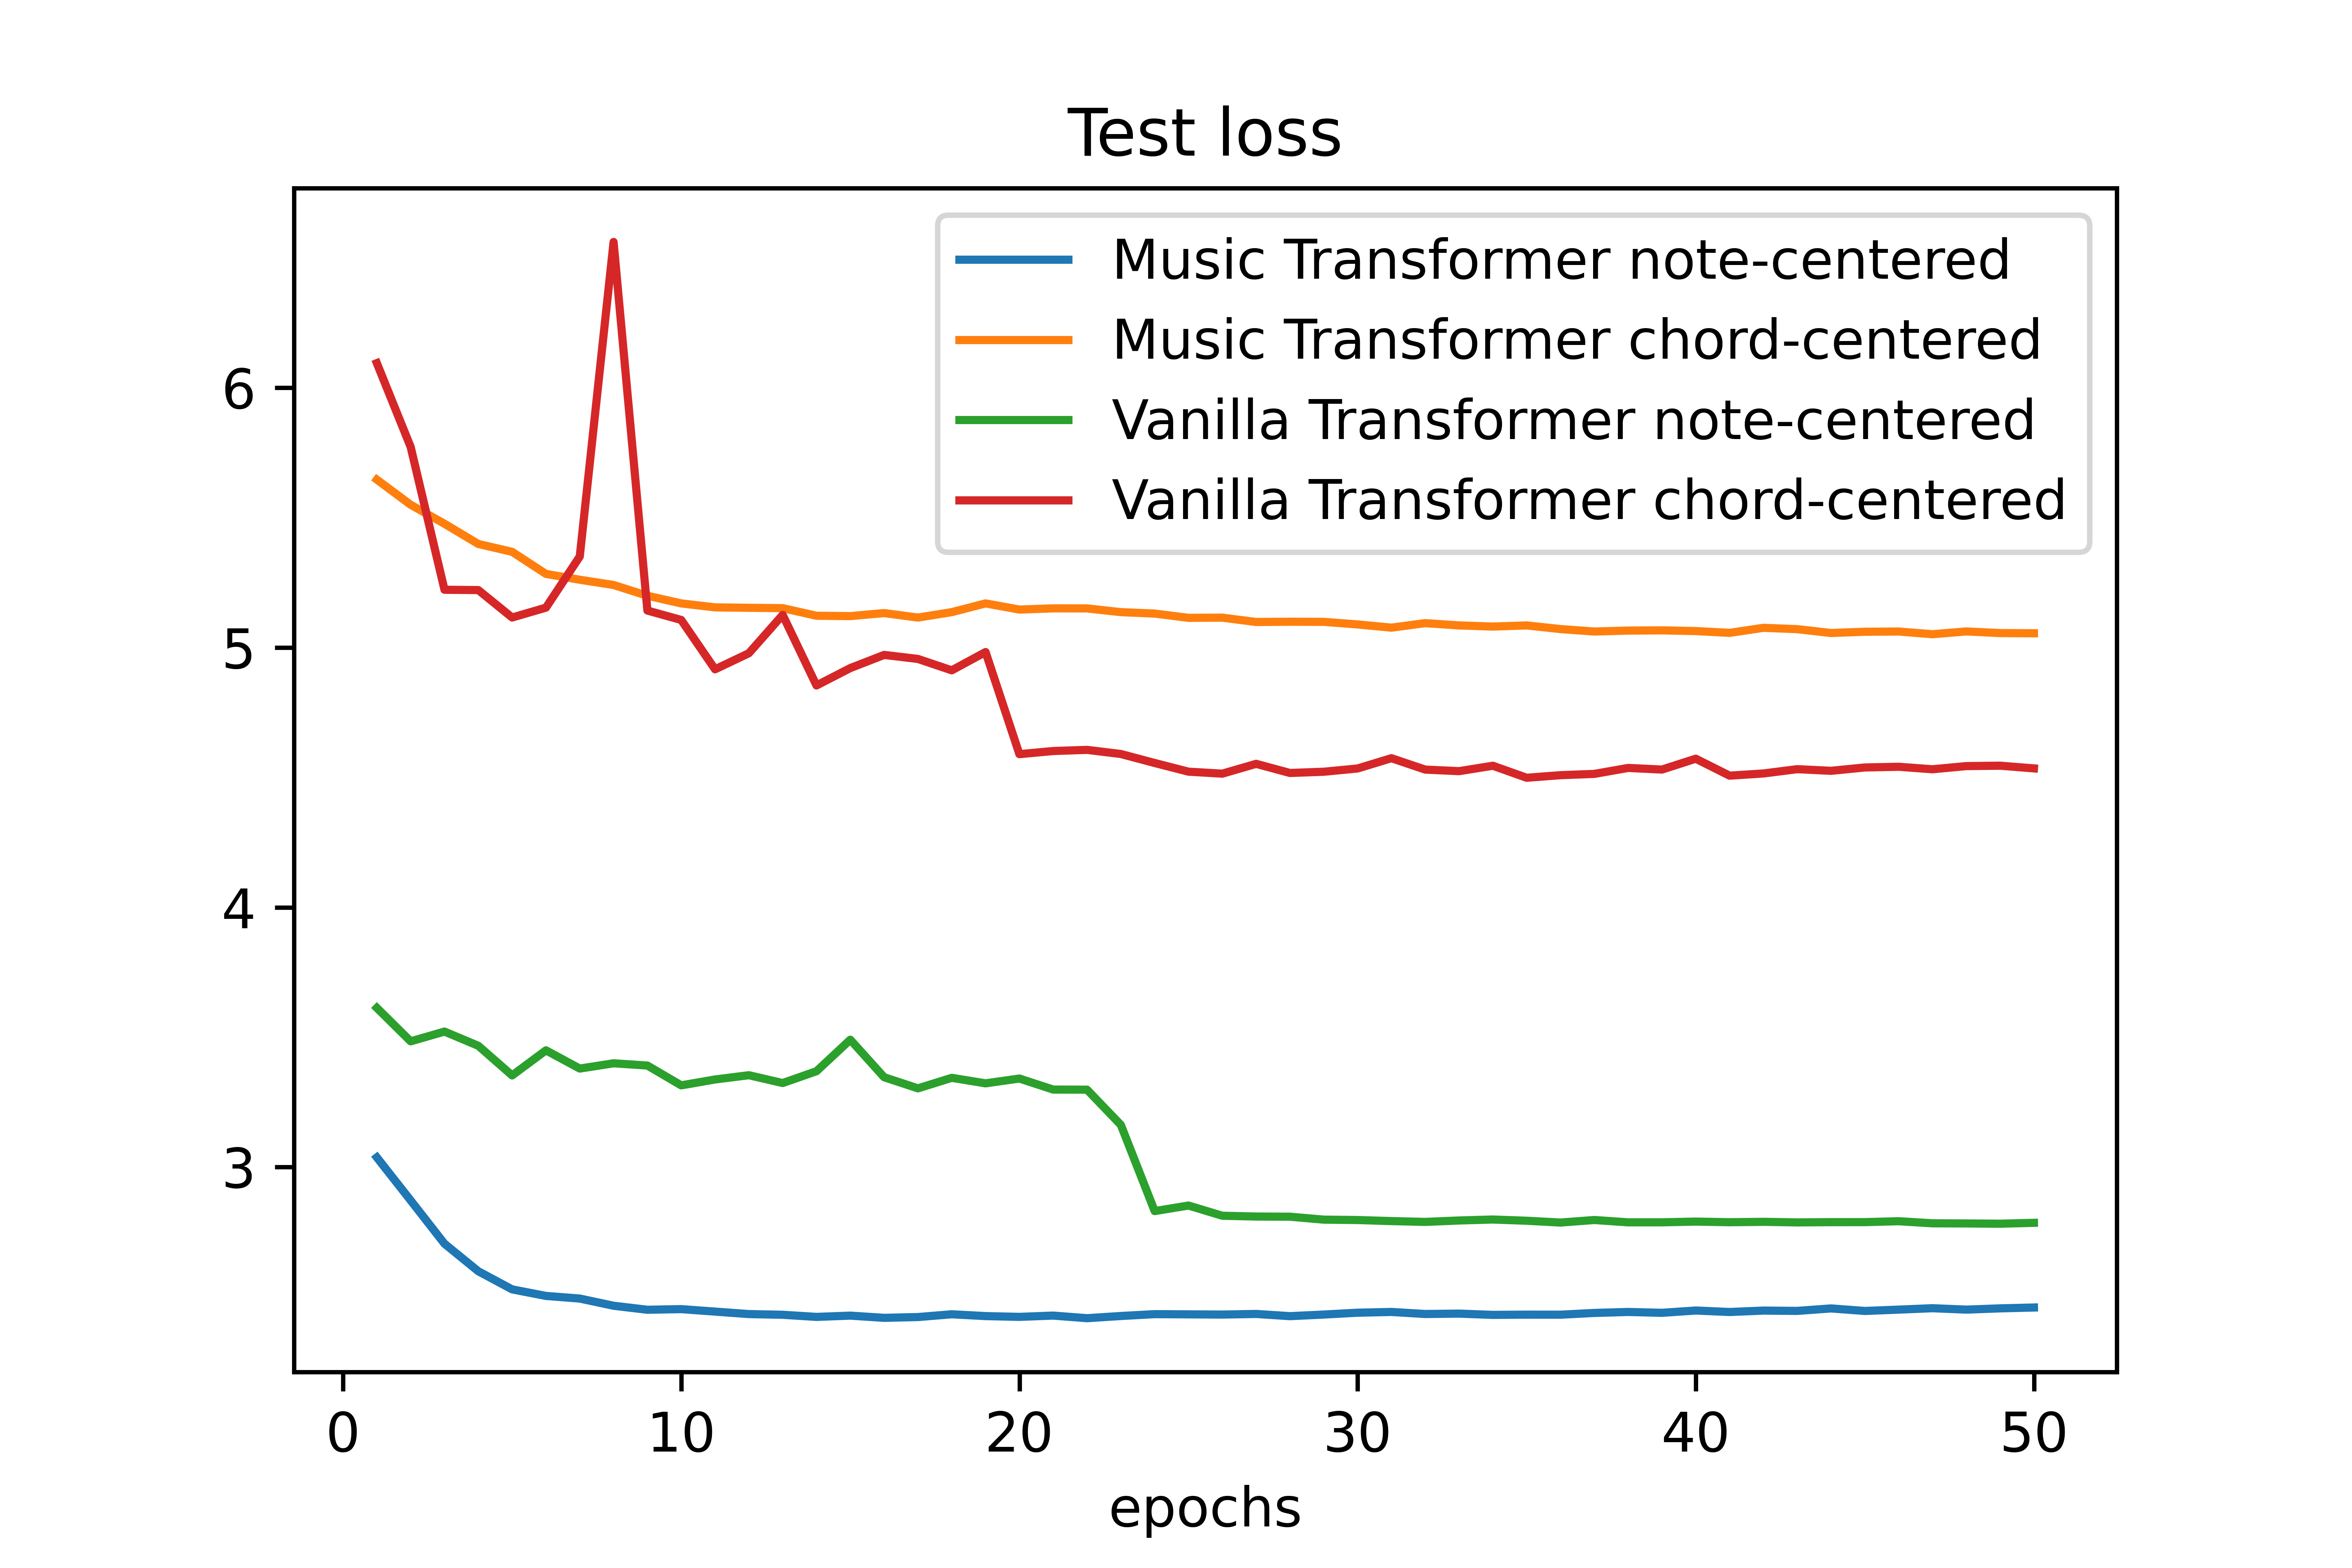
\includegraphics[width=0.8\textwidth]{assets/test-loss}
    \caption{~Loss of models on test set}\label{fig:appendix-test-loss}
\end{figure}

\begin{figure}
    \centering
    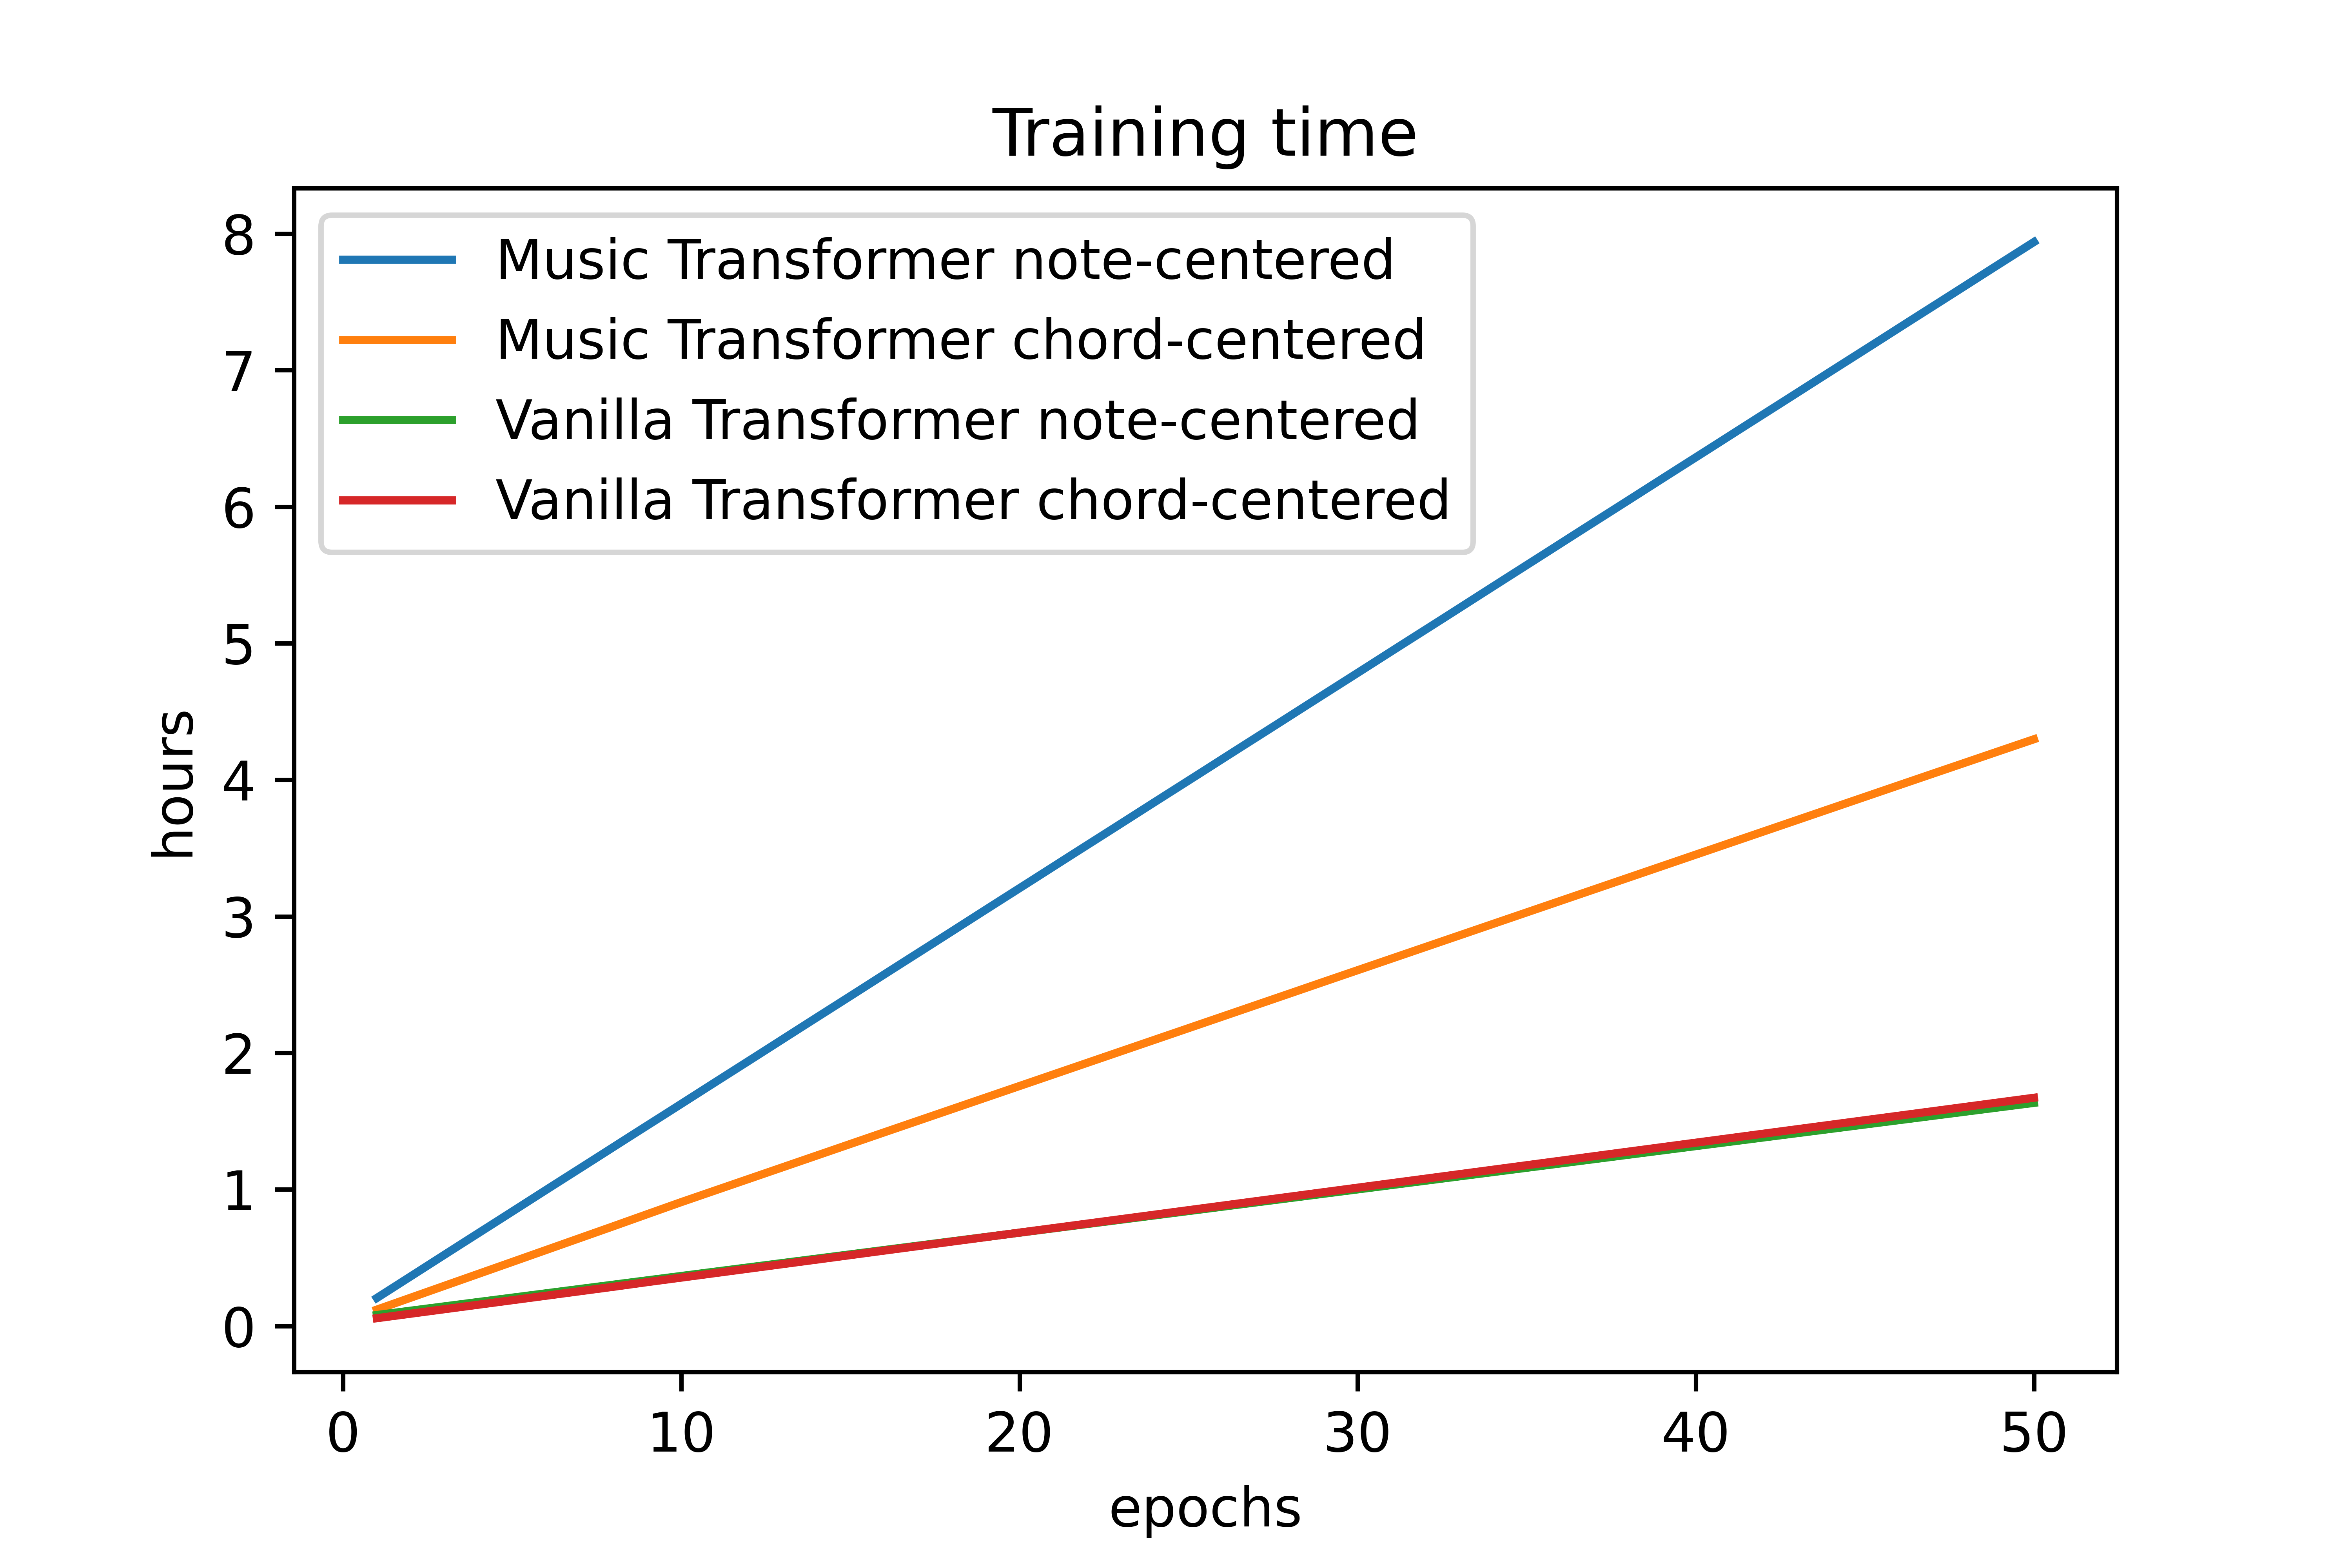
\includegraphics[width=0.8\textwidth]{assets/training-time}
    \caption{~Models training time}\label{fig:appendix-training-time}
\end{figure}